
\noindent\textbf{关于 (7.2.280.3) 的讨论。}
注意，同伦 (7.2.280.3) 是以下两个同伦的复合：
\begin{equation}
\begin{aligned}
\mathfrak g^{\psi_{1,s_0}\circ\phi}
&=j\circ\mathfrak f^{\psi_{1,s_0}\circ\phi}\\
&\sim j\circ
\mathfrak f_{\mathrm{ext},s=s_0}^{\psi_{1,s_0}}
\circ\mathfrak f^\phi,
\end{aligned}
\tag{7.2.330.1}\label{eq:7-2-330-1}
\end{equation}
\begin{equation}
\begin{aligned}
j\circ\mathfrak f_{\mathrm{ext},s=s_0}^{\psi_{1,s_0}}
\circ\mathfrak f^\phi
&\sim
j\circ\mathfrak f^{\psi_{1,s_0}}
\circ j\circ\mathfrak f^\phi\\
&=\mathfrak g^{\psi_{1,s_0}}\circ\mathfrak g^\phi.
\end{aligned}
\tag{7.2.330.2}\label{eq:7-2-330-2}
\end{equation}

先研究 (7.2.330.2)。
这部分与 (7.2.298.1) 平行。
首先得到
\[
C_d^{s=s_0}
(L'_1,((\lambda_0,\lambda_1),\lambda'_1))
\quad\text{及}\quad
\mathfrak f_{\mathrm{ext},s=s_0}^{\psi_{1,s_0}},
\]
使图式~\ref{diag:7-2-22} 交换。

\par\medskip\noindent\begin{minipage}{\textwidth}
\centering
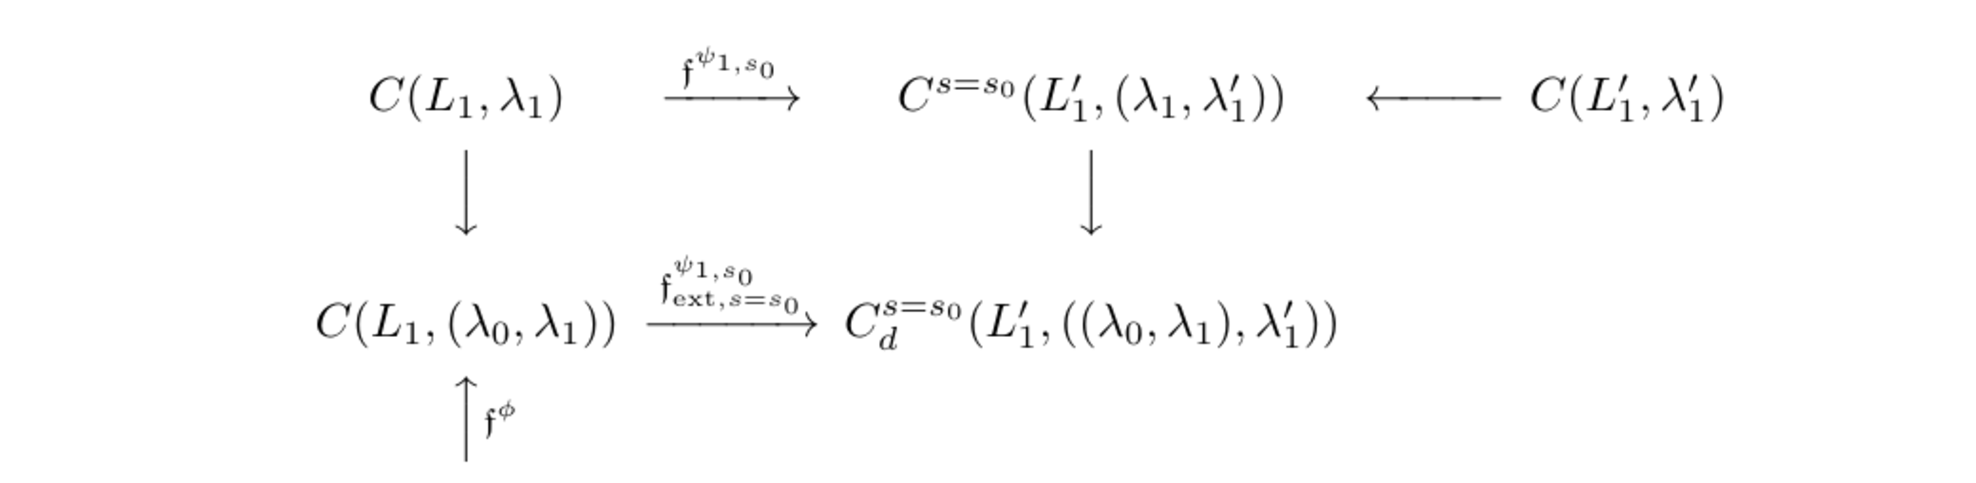
\includegraphics[width=\textwidth]{chapters/ch07-transversality/figures/phys-567-diagram-7-2-22-nocap.png}\\[0.4em]
{\renewcommand{\thefigure}{7.2.22}\refstepcounter{figure}
\normalfont\bfseries 图式~\thefigure\label{diag:7-2-22}}
\end{minipage}\par\medskip

再取其带 $s$ 参数的版本，得到如下对象：
\begin{itemize}
\item 滤过 $A_{n',K'}$ 代数
$C_d([0,1]_s\times L'_1,
((\lambda_0,\lambda_1),\lambda'_1))$\translatornote{原书此项写作无下标的
$C([0,1]_s\times L'_1,((\lambda_0,\lambda_1),\lambda'_1))$；
同一清单中的包含映射及图式 7.2.23、7.2.24
均以 $C_d$ 为相应对象。}
和 $C([0,1]_s\times L'_1,\lambda'_1)$；
\item 滤过 $A_{n',K'}$ 同态\translatornote{第一条包含映射的源在原书写成
$C(L_1,\lambda'_1)$；
依本段对象及图式 7.2.23 改为 $C(L'_1,\lambda'_1)$。}
\[
\begin{aligned}
\operatorname{Incl}\colon\;
&C(L'_1,\lambda'_1)
\longrightarrow C([0,1]_s\times L'_1,\lambda'_1),\\
\operatorname{Incl}\colon\;
&C(L_1,\lambda_1)
\longrightarrow C_d([0,1]_s\times L'_1,
((\lambda_0,\lambda_1),\lambda'_1));
\end{aligned}
\]
\item 各评价映射 $\operatorname{Eval}$，
以及
$\mathfrak f_{\mathrm{ext}}^{\{\psi_{1,s}\}_s}$。
\end{itemize}

它们满足下列性质：

\par\noindent\textup{(7.2.331.1)}
$\operatorname{Eval}$ 和 $\operatorname{Incl}$
满足 (7.2.175)。

\begin{equation}
\operatorname{Eval}_{s=s_0}\circ
\mathfrak f_{\mathrm{ext}}^{\{\psi_{1,s}\}_s}
=\mathfrak f_{\mathrm{ext},s=s_0}^{\psi_{1,s_0}}.
\tag{7.2.331.2}\label{eq:7-2-331-2}
\end{equation}

\par\noindent\textup{(7.2.331.3)}
图式~\ref{diag:7-2-23} 交换。

\par\medskip\noindent\begin{minipage}{\textwidth}
\centering
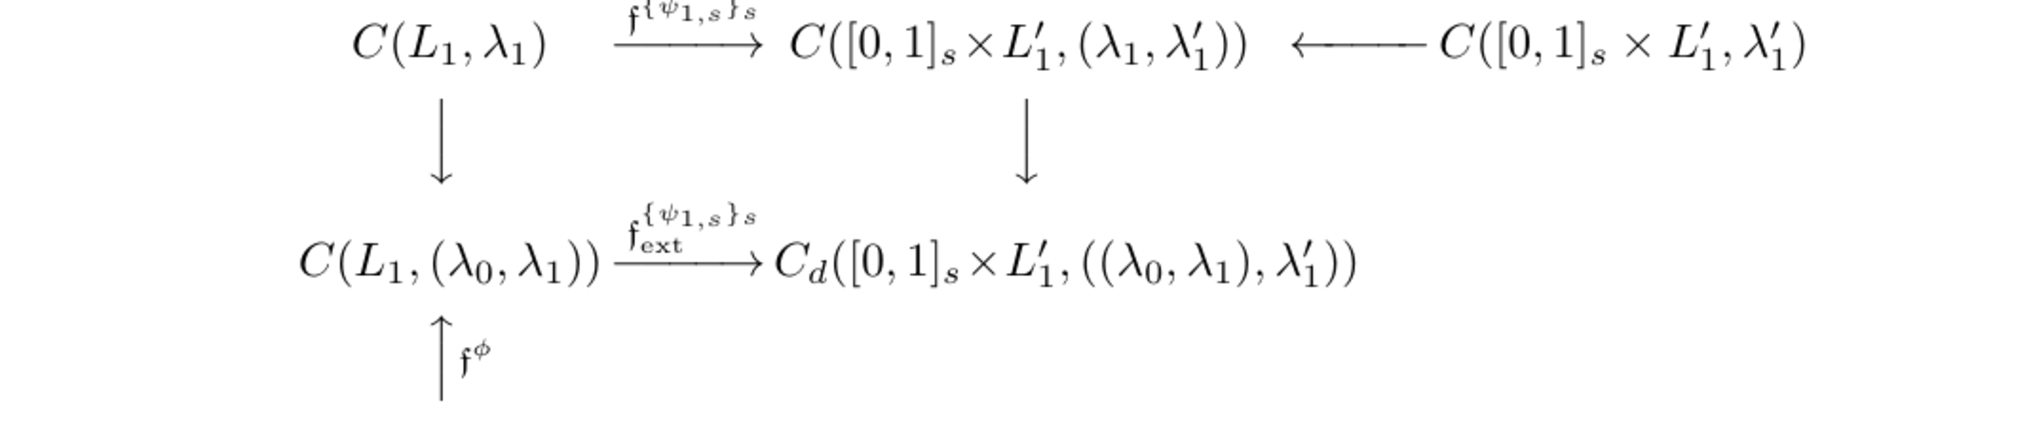
\includegraphics[width=\textwidth]{chapters/ch07-transversality/figures/phys-568-diagram-7-2-23-nocap.png}\\[0.4em]
{\renewcommand{\thefigure}{7.2.23}\refstepcounter{figure}
\normalfont\bfseries 图式~\thefigure\label{diag:7-2-23}}
\end{minipage}\par\medskip

注意 $C([0,1]_s\times L'_1,\lambda'_1)$
就是引理~\ref{lem:7-2-300}
中已引入的那个滤过 $A_{n',K'}$ 代数。

\begin{lemma}{7.2.332}\label{lem:7-2-332}
存在滤过 $A_{n',K'}$ 同态
$\mathfrak e_d$ 和 $\mathfrak E_d$，
满足下列性质：

\par\noindent\textup{(7.2.333.1)}
图式~\ref{diag:7-2-24}
在滤过 $A_{n,K}$ 同伦意义下交换。

\par\medskip\noindent\begin{minipage}{\textwidth}
\centering
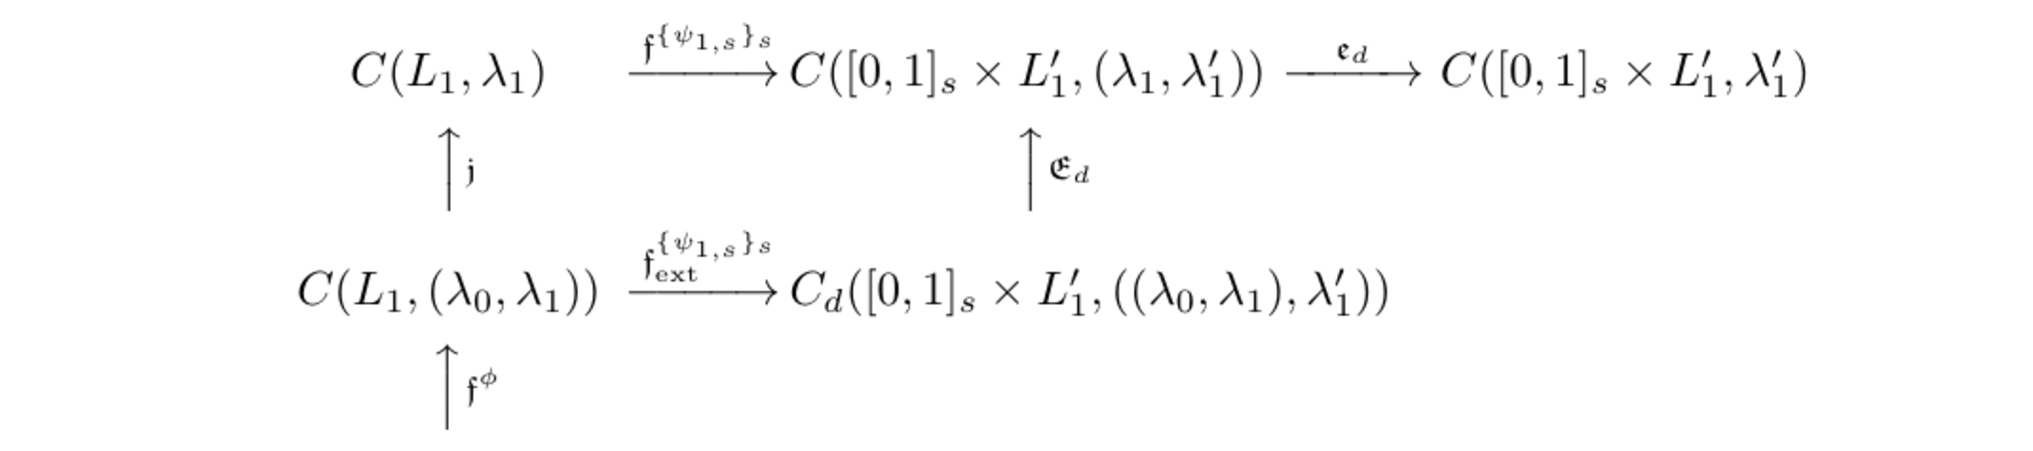
\includegraphics[width=\textwidth]{chapters/ch07-transversality/figures/phys-568-diagram-7-2-24-nocap.png}\\[0.4em]
{\renewcommand{\thefigure}{7.2.24}\refstepcounter{figure}
\normalfont\bfseries 图式~\thefigure\label{diag:7-2-24}}
\end{minipage}\par\medskip

\par\noindent\textup{(7.2.333.2)}
$\mathfrak e_d$ 在
$C([0,1]_s\times L'_1,\lambda'_1)$
上为恒等映射。

\par\noindent\textup{(7.2.333.3)}
$\mathfrak E_d$ 在
$C([0,1]_s\times L'_1,(\lambda_1,\lambda'_1))$
上为恒等映射。

\begin{equation}
\operatorname{Eval}_{s=s_0}\circ\mathfrak E_d
=j_{s=s_0}\circ\operatorname{Eval}_{s=s_0}.
\tag{7.2.333.4}\label{eq:7-2-333-4}
\end{equation}
\begin{equation}
\operatorname{Eval}_{s=s_0}\circ\mathfrak e_d
=j_{s=s_0}\circ\operatorname{Eval}_{s=s_0}.
\tag{7.2.333.5}\label{eq:7-2-333-5}
\end{equation}
这里的两个同名映射分别是
\[
\begin{aligned}
j_{s=s_0}\colon\;
&C_d^{s=s_0}
(L'_1,((\lambda_0,\lambda_1),\lambda'_1))
\longrightarrow C(L'_1,\lambda'_1),\\
j_{s=s_0}\colon\;
&C^{s=s_0}(L'_1,(\lambda_1,\lambda'_1))
\longrightarrow C(L'_1,\lambda'_1),
\end{aligned}
\]
它们是相应包含映射的同伦逆。
\end{lemma}

引理~\ref{lem:7-2-332} 可由障碍理论证明。

下面具体说明 (7.2.333.1) 中的同伦。
令
$\widehat{\mathfrak C}_d(L'_1,\lambda'_1)$
为
$[0,1]_r\times
C([0,1]_s\times L'_1,\lambda'_1)$
的一个模型。
更准确地说，取
\[
\widehat{\mathfrak C}_d(L'_1,\lambda'_1)
=C([0,1]_s\times L'_1,\lambda'_1)^{[0,1]_r}.
\]
于是，按照定义~\ref{def:7-2-188}，
$\widehat{\mathfrak C}_d(L'_1,\lambda'_1)$
是
$[0,1]^2\times C(L'_1,\lambda'_1)$
的模型。
其端面满足
\[
\begin{aligned}
\bigl(\widehat{\mathfrak C}_d(L'_1,\lambda'_1)\bigr)_{s=s_0}
&=\mathfrak C_{d,r}(L'_1,\lambda'_1),\\
\bigl(\widehat{\mathfrak C}_d(L'_1,\lambda'_1)\bigr)_{r=r_0}
&=C([0,1]_s\times L'_1,\lambda'_1),
\end{aligned}
\]
其中
\[
\mathfrak C_{d,r}(L'_1,\lambda'_1)
=C(L'_1,\lambda'_1)^{[0,1]_r}
\]
是 $[0,1]_r\times C(L'_1,\lambda'_1)$
的一个模型。

存在
\[
\operatorname{Incl}_r\colon
C([0,1]_s\times L'_1,\lambda'_1)
\longrightarrow\widehat{\mathfrak C}_d(L'_1,\lambda'_1),
\]
使
\begin{equation}
\operatorname{Eval}_{s=s_0}\circ\operatorname{Incl}_r
=\operatorname{Incl}_r\circ\operatorname{Eval}_{s=s_0}
\tag{7.2.334}\label{eq:7-2-334}
\end{equation}
成为从
$C([0,1]_s\times L'_1,\lambda'_1)$
到 $\mathfrak C_{d,r}(L'_1,\lambda'_1)$
的映射等式。

又有
\[
\mathcal F_d^{s=s_0}\colon
C(L_1,(\lambda_0,\lambda_1))
\longrightarrow
\mathfrak C_{d,r}(L'_1,\lambda'_1),
\]
满足以下端面式\translatornote{原书此处及后续证明均写连续两个
$j_{s=s_0}$；
但上述给出的两个同名映射均以
$C(L'_1,\lambda'_1)$ 为靶，
不能按所列型别直接复合。
此处保留原式，待进一步裁决。}：
\begin{equation}
\operatorname{Eval}_{r=0}\circ\mathcal F_d^{s=s_0}
=j_{s=s_0}\circ j_{s=s_0}\circ
\mathfrak f_{\mathrm{ext},s=s_0}^{\psi_{1,s_0}},
\tag{7.2.335.1}\label{eq:7-2-335-1}
\end{equation}
\begin{equation}
\operatorname{Eval}_{r=1}\circ\mathcal F_d^{s=s_0}
=j_{s=s_0}\circ\mathfrak f^{\psi_{1,s_0}}\circ j,
\tag{7.2.335.2}\label{eq:7-2-335-2}
\end{equation}
\begin{equation}
\mathcal F_d^{s=s_0}
=\operatorname{Incl}_r\circ j_{s=s_0}
\circ\mathfrak f^{\psi_{1,s_0}}
\quad\text{在 }C(L_1,\lambda_1)\text{ 上}.
\tag{7.2.335.3}\label{eq:7-2-335-3}
\end{equation}
换言之，
$\mathcal F_d^{s=s_0}\circ\mathfrak f^\phi$
给出同伦 (7.2.330.2)\translatornote{原书此处写
“同伦 (7.2.330.1)”；
但本段开头明确先研究 (7.2.330.2)，
且 (7.2.335.1)--(7.2.335.2)
的两端与 (7.2.330.2) 对应。}。
满足 (7.2.335.1) 和 (7.2.335.2)
的 $\mathcal F_d^{s=s_0}$ 之存在性，
来自把图式~\ref{diag:7-2-22} 中两支箭头
方向反转所得图式的同伦交换性。
而 (7.2.335.3)
来自该图式在 $C(L_1,\lambda_1)$
上的严格交换性。
